\section{Hardware}

% NOTE: The easiest way to find the hardware specifics of a device
%       is to run the deviceQuery executable (cuda-samples)
%   git clone https://github.com/NVIDIA/cuda-samples.git
%   cd cuda-samples
%   make -j 6
%   cd bin/x86_64/linux/release
%   ./deviceQuery


% NOTE 2:
%  Ampere A100:
%    https://images.nvidia.com/aem-dam/en-zz/Solutions/data-center/nvidia-ampere-architecture-whitepaper.pdf
%    https://developer.nvidia.com/blog/nvidia-ampere-architecture-in-depth/

%  Hopper H100:
%    https://developer.nvidia.com/blog/nvidia-hopper-architecture-in-depth/

%  Blackwell B100:
%    https://resources.nvidia.com/en-us-blackwell-architecture

%  Will be succeeded by the Rubin generation (R100/R200)
%    https://blogs.nvidia.com/blog/computex-2024-jensen-huang/

\subsection{Streaming multiprocessor (SMP)}
\begin{frame}
\frametitle{Streaming Multiprocessor (SMP)}
\begin{itemize}
\item GPU device connected to the CPU by a PCIe bus. 
\item each GPU device contains an array (\textcolor{red}{$\mathbf{x}$}) of Streaming Multiprocessors \textbf{(SMP)}.
\item each SMP has:
\begin{itemize}
   \item a Single-Instruction Multiple-Thread (\texttt{SIMT}) Architecture.
   \item contains \textcolor{red}{$\mathbf{y}$} regular cores and [\textcolor{red}{$\mathbf{z}$} tensor cores].
\end{itemize} 
\item scalable: newer generations: increase of \textcolor{red}{$\mathbf{x}$}, \textcolor{red}{$\mathbf{y}$} 
	and [\textcolor{red}{$\mathbf{z}$}], e.g.:
   \begin{itemize}
	   \item \texttt{NVIDIA A100-PCIE-40GB} (\textit{notch293})
         \begin{itemize}
            \item global memory: $40$ GB.			 
            \item $108$ SMPs, $64$ Cores/SMP, $4$ Tensor Cores/SMP.
            \item GPU Max. Clock Rate: $1.41$ GHz.
         \end{itemize}		   
 \item \texttt{NVIDIA H100 SXM5 NVL} (\textit{grn008})	
         \begin{itemize}
            \item global memory: $93$ GB.			 
            \item $132$ SMPs, $128$ Cores/SMP, $4$ Tensor Cores/SMP.
	    \item GPU Max. Clock Rate: $1.78$ GHz. 
         \end{itemize}
   \end{itemize}		   
\end{itemize}
\end{frame} 

% NOTE: 
\begin{frame}
	\frametitle{\texttt{NVIDIA GH100 SMP}} 
    \begin{columns}
	\column{0.50\textwidth}
    \begin{figure}[H]
       \centering
	    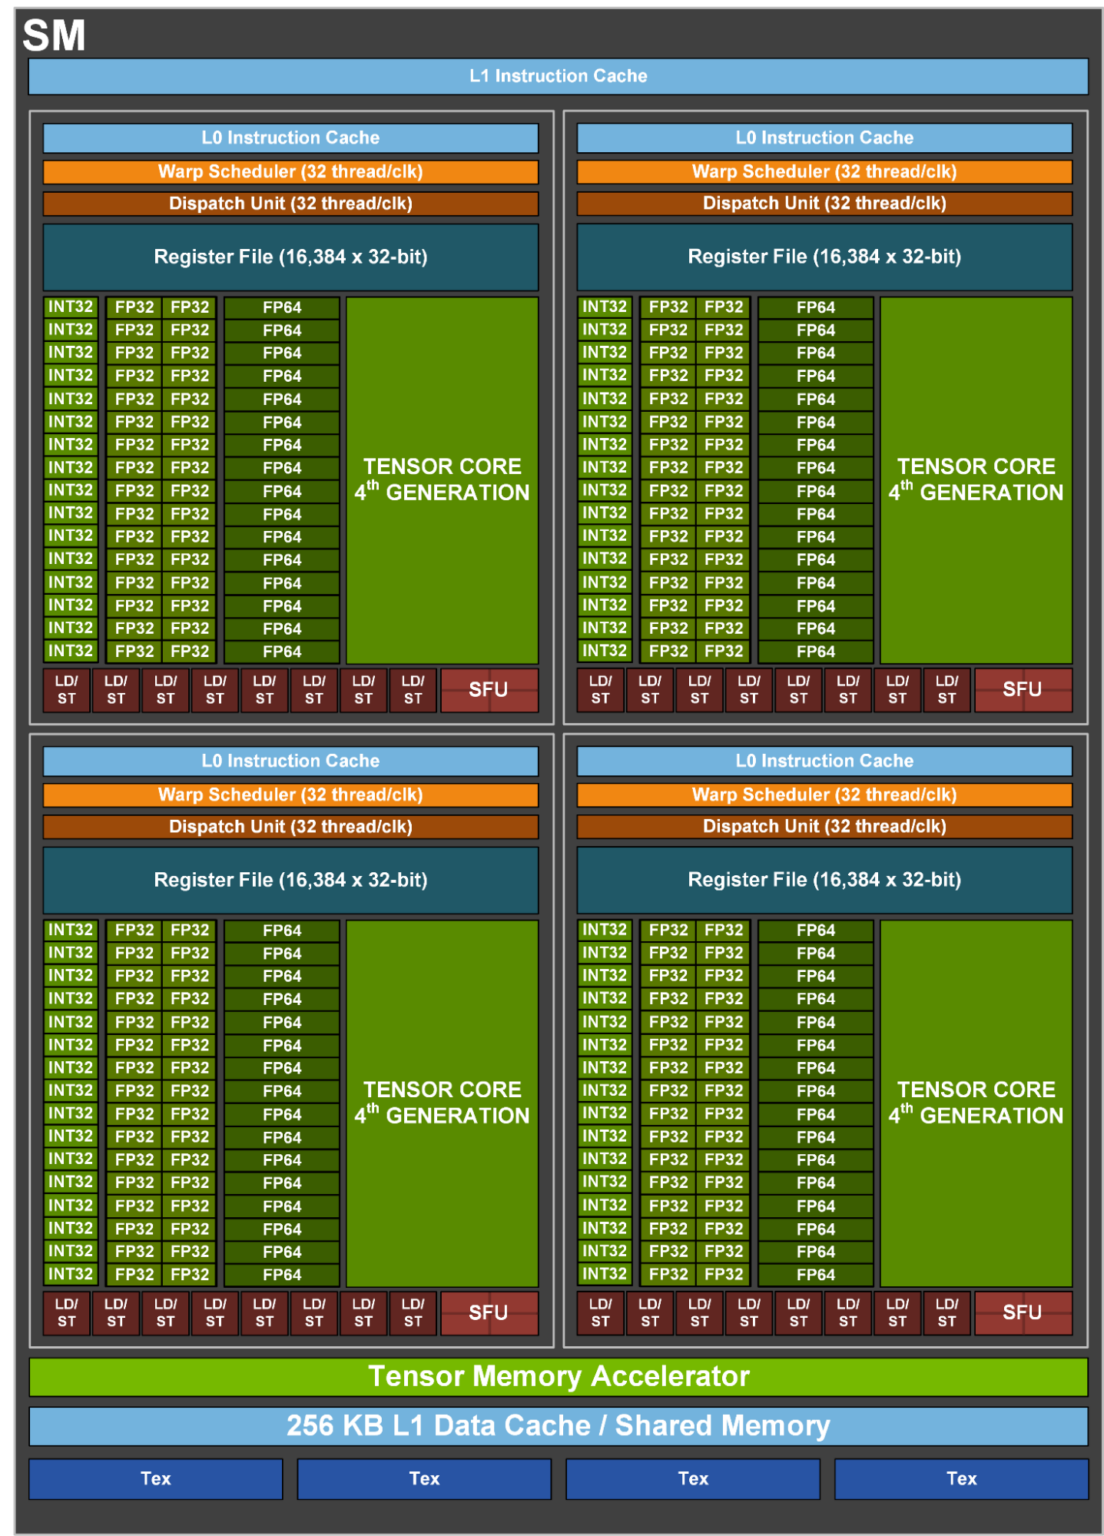
\includegraphics[width=0.80\textwidth]{./img/H100-Streaming-Multiprocessor-SM-1104x1536.png}
	    \caption{\small{GH100 SMP.}}
     \end{figure}
     \end{columns}
\end{frame}

\begin{frame}
        \frametitle{\texttt{NVIDIA GH100 Full Device}}
    \begin{columns}
        \column{0.90\textwidth}
    \begin{figure}[H]
       \centering
	    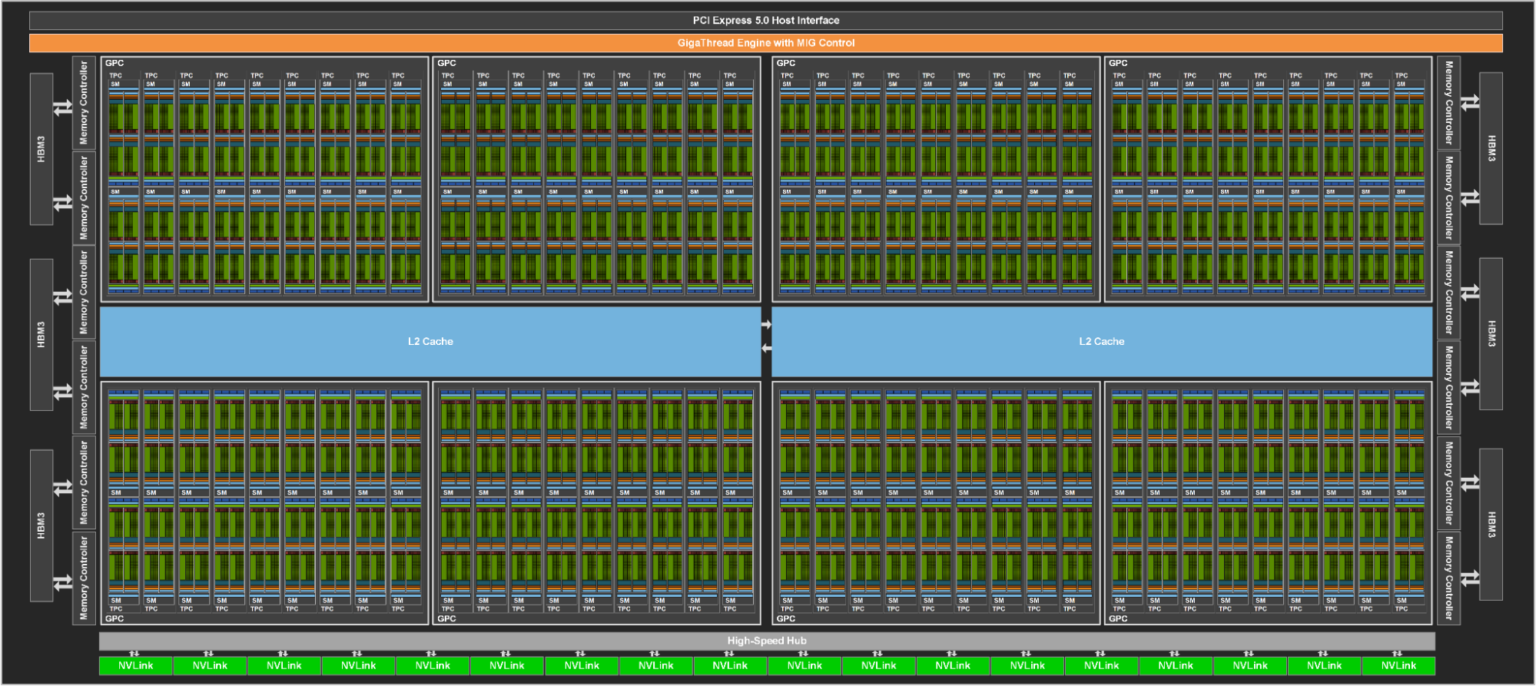
\includegraphics[width=0.90\textwidth]{./img/Full-H100-GPU-with-144-SMs-1536x686.png}
	    \caption{\small{NVIDIA GH100 Full Device ($144$ SMPs).}}
     \end{figure}
     \end{columns}
\end{frame}

\subsection{Warps}
\begin{frame}
\frametitle{GPU Threads - Warps}	
\begin{itemize}
  \item Each SMP:	
  \begin{itemize}
     \item generates, schedules, executes threads in batches of $32$ threads.
     \item \textbf{WARP}: a batch of $32$ threads
  \end{itemize}
  \item each thread in a WARP executes the same instructions but runs its own "path".
  \item if threads within a WARP diverge, the threads become inactive/disabled.
\end{itemize}	   
\end{frame} 

\subsection{Types of GPU memory}
\begin{frame}
\frametitle{Types of GPU memory}
\begin{itemize}
  \item global memory (largest and slowest)
  \item shared memory: allocated per thread block \& low latency
  \item constant memory: cached, read-only
  \item registers: fast, on-chip memory (exclusive to each thread).
\end{itemize}	  
\end{frame}


